
\label{sec:introduction}

The advent of multicore architectures has made multithreaded
programming increasingly necessary, but writing multithreaded programs remains painful. It is notoriously far more challenging to write concurrent programs than sequential ones because of the wide range of errors it can cause, including deadlocks and race conditions~\cite{havender,76897,130623}. Because thread interleavings are non-deterministic, different runs of the same multithreaded program can unexpectedly produce different results. These ``Heisenbugs'' greatly complicate debugging, and eliminating them requires extensive testing to account for possible thread interleavings~\cite{DBLP:conf/icse/BallBHMQ09,DBLP:conf/asplos/BurckhardtKMN10}.


Instead of testing, one promising alternative approach is to attack the problem of concurrency bugs by eliminating its source: non-determinism. A fully \emph{deterministic multithreaded system} would prevent Heisenbugs by ensuring that executions of the same program with the same inputs always yield the same results, even in the face of race conditions in the code. Such a system would not only dramatically simplify debugging of concurrent programs~\cite{Carver:1991:RTC:624586.625040} and reduce their attendant testing overhead, but would also enable a number of other applications. For example, a deterministic multithreaded system would greatly simplify record and replay for multithreaded programs~\cite{Choi:1998:DRJ:281035.281041,LeBlanc:1987:DPP:32387.32396}
and the execution of multiple replicas of multithreaded applications for fault tolerance~\cite{deterministic-process-groups,1134000,224058,replicant-hotos}.

Several recent software-only proposals aim at providing
deterministic multithreading, but these all suffer from a variety of disadvantages. Language-based approaches are effective at removing determinism but require programmers to write code in specialized languages, which can be impractical~\cite{Bocchino:2009:TES:1640089.1640097,Burckhardt:2010:CPR:1869459.1869515,Simpson:1999:SEE:330346.330357}. Recent deterministic systems that target legacy programming languages
(especially C/C++) are either incomplete or impractical. Kendo ensures determinism of synchronization operations with low overhead, but does not guarantee determinism in the presence of data races~\cite{1508256}. Grace prevents all concurrency errors but is limited to fork-join programs, and although it is efficient, it can require code modifications to avoid large runtime overhead~\cite{grace}. CoreDet, a compiler and runtime system, enforces deterministic execution for arbitrary multithreaded C/C++ programs~\cite{Bergan:2010:CCR:1736020.1736029}. However, it exhibits prohibitively high overhead (running up to $8\times$ slower than \pthreads{}; see Section~\ref{sec:evaluation}) and generates thread interleavings at arbitrary points in the code, complicating program debugging and testing.

\hspace{1em} \\
\noindent
\textbf{Contributions:}
This paper presents \textbf{\dthreads{}}, an efficient deterministic runtime system for multithreaded C/C++ applications. \dthreads{} guarantees deterministic execution of multithreaded programs even in the presence of data races (notwithstanding external sources of non-determinism
like I/O): given the same sequence of inputs, a program
using \dthreads{} always produces the same output. \dthreads{}'
deterministic commit protocol not only eliminates data races but also prevents lock-based deadlocks.

\dthreads{} is easy to deploy: it works as a direct replacement for the \pthreads{} library, requiring no code modifications or
recompilation. \dthreads{} is also efficient. \dthreads{} leverages process isolation and virtual memory protection to track and isolate concurrent memory updates, which it deterministically commits. Not only does this approach greatly reduce overhead versus approaches that use software read and write barriers, it also eliminates cache-line based false sharing, a notorious performance problem for multithreaded
programs. These two features combine to enable \dthreads{} to nearly match or even exceed the performance of \pthreads{} for the majority of the benchmarks examined here. \dthreads{} thus marks a significant improvement over the state of the art in deployability and performance, and provides promising evidence that fully deterministic multithreaded programming may be practical.

\section{\dthreads{} Overview}
Figure~\ref{fig:nondeterminism} shows an example multithreaded program that, because of data races, non-deterministically produces the outputs ``1,0,'' ``0,1,'' and ``1,1.''  The order of instructions are changed from one execution to the other, resulting in these nondeterministic outputs. Using \dthreads{}, this program will \emph{deterministically} produce the same output-``1,1'' . Although this output can be a undesired one, the fact that results are always reproducible would make it easy for developers to reproduce and locate data races inside parallel programs.

\begin{figure}[h]
{\centering
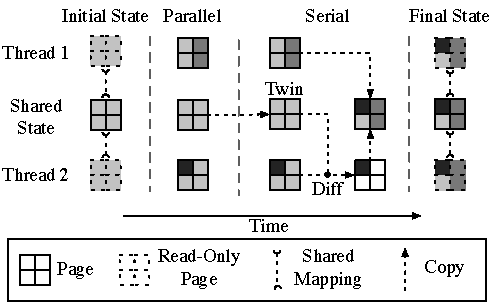
\includegraphics[width=6in]{dthreads/figure/architecture-diagram}
\caption{An overview of \dthreads{} execution.\label{fig:architecture}}
}
\end{figure}

\dthreads{} employs the following mechanisms to ensure the deterministic execution, illustrated by Figure~\ref{fig:architecture}: 

\textbf{Isolated Memory Access:} In \dthreads{}, threads are actually running as separate processes with private and shared views of memory, which is based on the \sheriff{} framework. Because processes have separate address spaces, \dthreads{} can isolate executions of different ``threads''. \dthreads{} uses this isolation mechanism to control the visibility of memory state, so that the updates made by a thread can not be seen by other threads if those updates are not committed explicitly to the shared mapping. By doing this, we guarantee that each ``thread'' can operate independently until synchronization points. Implementation of this is discussed in depth in Section~\ref{sec:threadsasprocs}.

\textbf{Deterministic Memory Commit:} 
Multithreading programs use shared memory for communication, thus \dthreads{} must propagate a thread's changes to be seen by other threads. To guarantee determinism, \dthreads{} should publish updates of different threads in a deterministic order at deterministic points.

\dthreads{} actually commits the changes of a thread to the shared state in sequence at synchronization points. These points includes thread creation and exit; mutex lock and unlock; condition variable wait and signal; posix sigwait and signal; and barrier waits. Commits are ordered using a global ``token'' that is passed from one thread to the next; a thread can only commit when it holds the token.  The token-passing protocol is described in Section~\ref{sec:schedule} and the implementation of synchronization primitives is described in Section~\ref{sec:synchronization}.

\dthreads{} relies on the twinning and diffing mechanism to find out local changes of different threads, which has been discussed in Section~\ref{sec:twinning-and-diffing}. 

\textbf{Deterministic Synchronization:}
There is no deterministic guarantee on synchronizations under existing operating systems. Thus, \dthreads{} re-implements the full range of pthreads synchronization primitives and discusses  them in details in Section~\ref{sec:synchronization}. 

\hspace{1em} \\
\noindent
\textbf{Fixing the data race example} \\
About the example program in Figure~\ref{fig:nondeterminism},  \dthreads{} effectively isolates the execution from each thread until it completes, and then orders updates from different threads by thread creation time using a deterministic last-writer-wins protocol.

In the beginning of every execution, thread 1 and thread 2 have the same view of shared state, with a = 0 and b = 0. Because changes by one thread to the value of a or b will not be made visible to the other until this thread exits, both checks on two threads on line 2 will be true. Thread 1 sets the value of a to 1, and thread 2 sets the value of b to 1. These threads then commit their updates to the shared state and exit, with thread 1 always committing before thread 2. The main thread then should always prints “1, 1” on every execution.

This determinism not only enables record-and-replay and replicated execution, but also effectively converts Heisenbugs into “Bohr” bugs, making them reproducible. In addition, \dthreads{} optionally reports any conflicting updates due to racy writes, further simplifying debugging.


\section{\dthreads{} Architecture}

\begin{comment}
Because multithreaded programs frequently use updates to shared memory to communicate, \dthreads{} must implement a mechanism to expose one thread's updates to all other threads.  At the beginning of a transaction, all shared pages are protected, and can only be read by threads.  When a thread attempts to modify a shared page a local working copy is created, leaving the shared page unmodified.  At commit time, a ``twin'' copy of all modified pages is created.  Every page is compared to its twin (using a byte-wise diff) and modified bytes are copied back to the shared state.  Unlike transactional memory, conflicting changes do not result in rollbacks with \dthreads{}.  Further details are described in Section~\ref{sec:sharedmemory}.
\end{comment}


\label{sec:dthreads-architecture}
This section describes \dthreads{}’ key algorithms—memory isolation, deterministic (diff-based) memory commit, deterministic synchronization, and deterministic memory allocation—as well as other implementation details.

\subsection{Isolated Memory Access}
\label{sec:threadsasprocs}

In order to achieve the deterministic memory access, 
\dthreads{} isolates memory accesses among different
threads between commit points, and commits the updates of each thread deterministically. \dthreads{} is based on the \sheriff{} framework, discussed in Section~\ref{sec:sheriffframework}.

Relying on the \sheriff{} framework, \dthreads{} isolates  memory access among different threads: different threads can only see their own local changes. Additionally, \dthreads{} shims the \texttt{getpid()} function to return a single, globally-shared process identifier. 

\subsubsection{Deterministic Thread Index}
\label{sec:threadindex}

POSIX does not guarantee deterministic process or thread identifiers. To avoid exposing this nondeterminism to threads running as processes, \dthreads{} shims the \texttt{pthread\_self()} function in order to return an internal thread index.  This internal thread index is managed using a single global variable that is incremented on thread creation.  This unique thread index is also used to manage per-thread heaps and as an offset into an array of thread entries.

\subsubsection{Shared Memory}
\label{sec:stackandheap}

In order to create the illusion that different threads are sharing the same address space, \dthreads{} uses memory mapped files to share the globals and heap across different processes.

As discussed in Section~\ref{sec:sharedmemory}, \dthreads{} creates two different mappings for both the heap and the globals.  One is a shared mapping, which is used to hold shared state. The other is a private, copy-on-write (COW) per-process mapping that each process works on directly.  Private mappings are linked to the shared mapping through the single fixed-size memory mapped file. Reads initially go directly to the shared mapping,
but after the first write operation, both reads and writes are entirely private.

Memory allocations are issued from the shared heap memory using a scalable per-thread heap organization loosely based on Hoard~\cite{BergerMcKinleyBlumofeWilson:ASPLOS2000} and built using HeapLayers~\cite{BergerZornMcKinley:2001}.  \dthreads{} divides the heap into a fixed number of sub-heaps (currently 16).  Each thread uses a hash of its thread index to find the appropriate sub-heap.

\subsection{Deterministic Memory Commit}
\label{sec:sharedmem}

\begin{figure}
{\centering 
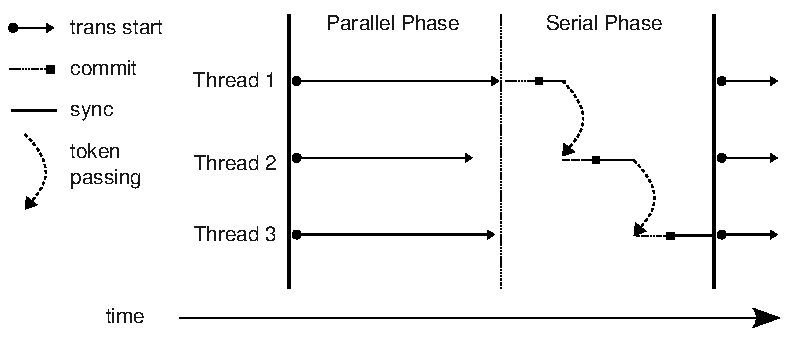
\includegraphics[width=3.25in]{dthreads/figure/phase}
\caption{An overview of \dthreads{} phase. Program execution with \dthreads{} alternates between parallel and serial phases.\label{fig:phase}}
}
\end{figure}

Figure~\ref{fig:phase} illustrates the execution of programs under \dthreads{}.  To guarantee determinism, \dthreads{} isolates memory accesses in parallel phases. In parallel phases, memory accesses work on private copies after the first write operation and updates are not shared across threads.  When a synchronization point is reached, updates are exposed in deterministic order.  This section describes the mechanisms used to guarantee deterministic commit order, and the details of commits to shared memory.

\subsubsection{Fence and Token}
\label{sec:schedule}

\dthreads{} places internal fences between the parallel and serial phases. \dthreads{} re-implements the fence because the standard \pthreads{} barrier mechanism does not support dynamic changes of threads number. 

\begin{figure}
\begin{lstlisting} [style=tt]
void waitFence(void) {
  lock();
	
  while(!isArrivalPhase()) { 
    CondWait();
  }

  waiting_threads++;
  if(waiting_threads < alive_threads) {
    while(!isDeparturePhase()) {
      CondWait();
    }
  } 
  else {
    setDeparturePhase();
    CondBroadcast();
  }

  waiting_threads--;
  if (waiting_threads == 0) {
    setArrivalPhase();
    CondBroadcast();
  }

  unlock();
}

\end{lstlisting}
\caption{Pseudocode for the internal fence.\label{fig:internalFence}}
\end{figure}

Figure~\ref{fig:internalFence} shows the pseudocode code for the internal fence. Threads must wait at the fence until all threads from the previous fence have departed. Then those threads are waiting on the fence until all alive threads  have entered into the same fence(lines 8-11). 
The last thread entering the fence initiates the departure phase and wakes up all threads on the fence(lines 14-15). As threads leave the fence, they decrement the waiting thread count.  The last thread to leave sets the fence to the arrival phase and wakes any waiting threads (lines 19-21).

To reduce overhead, whenever the number of running threads is
less than or equal to the number of cores, waiting threads block by spinning rather than by invoking relatively expensive cross-process \pthreads{} mutexes. When the number of threads exceeds the number of cores, \dthreads{} falls back to using \pthreads{} mutexes.

\begin{figure}
\begin{lstlisting} [style=tt]
void waitToken() {
  waitFence();
  while(isNotMyToken()) { yield(); }
}
void putToken() {
  passTokenToNextOfTokenQueue();
}
\end{lstlisting}
\caption{Pseudocode for waitToken and putToken. 
\label{fig:token}}
\end{figure}

Another key mechanism of \dthreads{} is using the token to order memory commits and synchronizations. The token implementation is listed in Figure~\ref{fig:token}. The token is a shared pointer that points to the next runnable thread entry, which guarantees the global order for all operations in serial phases.  

\dthreads{} introduces two subroutines to manage tokens.  The\texttt{waitToken()} function first waits at the internal fence and then waits to acquire the global token
in order to enter serial mode. The \texttt{putToken()} function passes the token to the next waiting thread. 

As shown in Figure~\ref{fig:phase}, it is very important for a thread to wait at the internal fence before a thread enters into serial phases or before a thread leaves serial phases, even for a thread that is guaranteed to have the token next. Memory commits by a thread can affect other threads' behavior. 

\subsubsection{Commit Protocol}
\begin{figure}
{\centering
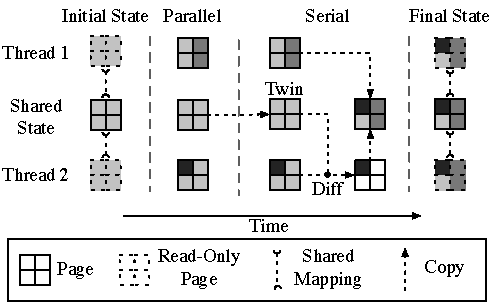
\includegraphics[width=5in]{dthreads/figure/architecture-diagram}
\caption{An overview of \dthreads{} execution.\label{fig:architecture}}
}
\end{figure}

Figure~\ref{fig:architecture} shows the steps to capture modifications to shared state and expose them in a deterministic order.  

At the beginning of the parallel phases, different threads have a read-only mapping for all shared pages. If a thread writes to a shared page during the parallel phases, this write is trapped in order to create a private copy and a twin page for this shared page. After that, reads and writes on this page happen on the private copy only. Reads go directly to the shared memory and are not trapped.  

In the serial phases, threads first commit their local changes happening in parallel phases one at a time, guided by the global token.  The first thread to commit to a page can directly copy its private copy to the shared state, but subsequent commits must copy only the modified bytes. To find out those modifications, \dthreads{} compares those private copies against those twin pages, creating from the shared mapping before actual modification.  After a thread commits its local changes, it issues synchronizations before it passes the token to next thread. 

In the end of serial phase, every threads have to wait at the fence in order to enter into the next parallel phase. 

\subsection{Deterministic Synchronization}
\label{sec:synchronization}
\dthreads{} supports the full range of synchronizations of
\pthreads{} APIs, including locks, conditional variables, barriers and different types of thread exit. Because the \sheriff{} framework can not provide any determinism guarantee, \dthreads{} re-implements all synchronizations as the following.

\subsubsection{Locks}
\dthreads{} uses the global token to guide synchronizations during the serial phases. Before a thread is acquiring a lock while current thread does not have the token, it has to wait for the global token. 

\dthreads{} treats multiple locks as the same one, which  possibly compromise the efficiency of programs, it only ends the serial phases when all locks are unlocked. Thus, it is possible for a program with deadlock problems that those deadlock do not occur to \dthreads{} at all. 

For the acquisitions of locks, \dthreads{} checks at first 
whether the current thread is already holding any locks. If not, the thread first waits for the token, commits those changes happened in the last parallel phase to shared state, and begins a new atomic section. Finally, the thread increments the number of locks it is currently holding. The lock count ensures that a thread does not pass the token to the next one until it has released all of the locks.

During the releases of locks, \dthreads{} decrements the lock count at first. A thread does nothing if there are still some locks holding by the current thread, with the lock count not equal to 0. If all locks have been released, \dthreads{} commits the memory changes happened in this serial phase to the shared mapping. Then it passes the global token to the next thread of the token queue and starts a new atomic region. Finally, the thread waits on the internal fence before entering into the next round's parallel phase.

\subsubsection{Condition Variables}
\label{sec:condwait}

Guaranteeing determinism for condition variables is much more complex than for other synchronization operations. The underlying operating system can not guarantee that threads are going to be waken-up in the same order as they wait on a conditional variable. Thus, a naive implementation easily leads to a deadlock problem.

% pthread_cond_wait: waiting threads are extracted from the 
% the token queue.
% Reducing the performance cost, 
When a thread calls \texttt{pthread\_cond\_wait}, it first acquires the global token and commits local modifications. It then removes itself from the token queue since threads waiting on condition variables do not participate in the token pass of the serial phase until they are awakened. Then, \dthreads{} adds itself to the conditional variable's waiting queue, decreases the alive thread count (used in the internal fence mechanism), and passes the token to the next thread on the token queue before actually waiting on a real process-shared conditional variable. When a thread is awaken, it should check at first whether the current thread is ready to run or not. For threads waken up by \texttt{pthread\_cond\_signal}, only the first thread in the waiting list can run in order to guarantee the First-In-First-Out order. All threads can run if waken up by \texttt{pthread\_cond\_broadcast}. If a thread is not able to run, it waits on the conditional variable again. If a thread is the candidate thread to be waken up, it waits for the global token because a thread waking up from a conditional variable is supposed to acquire the mutex, which means that it should already have the global token. 

For those waken-up functions, including \texttt{pthread\_cond\_signal} and \texttt{pthread\_cond\_broadcast}, the calling thread first waits for the token, and then commits any local modifications. If no threads are waiting on the condition variable, \dthreads{} passes the token to the next thread immediately. Otherwise, \dthreads{} moves corresponding threads in the condition variable queue to the head of the token queue, marked them as ready, and increments the live thread count correspondingly. To guarantee that threads are waken-up in the same order as they wait on a conditional variable, \texttt{pthread\_cond\_signal} only do this for the first thread in the queue but \dthreads{} wakes up all threads simultaneously. Those not-ready threads immediately wait again after waken-up. In order to improve the performance, those newly waken-up threads are scheduled to run next by simply putting them into the header of the token queue so that the calling thread can pass the token to them. 


\subsubsection{Barriers}

\label{sec:barrierwait}

\dthreads{} must ensure that threads waiting on a barrier do not disrupt the token passing of running threads. \dthreads{} removes threads entering into the barrier from the run queue and places them on the corresponding barrier queue.

In order to ensure the deterministic commit, the calling thread first waits for the global token to commit any local modifications. If the current thread is the last one to enter the barrier, \dthreads{} moves all threads on the barrier queue to the token queue, increases the alive threads count, and passes the token to the first thread in the barrier queue.  Otherwise, \dthreads{} removes the current thread from the token queue, places it on the barrier queue, releases the token. and waits on the actual barrier.


\subsubsection{Thread Creation and Exit}

\label{sec:threadcreation}

\begin{figure}
\begin{lstlisting} [style=tt]
void thread_create () {
  waitToken();
  clone(CLONE_FS| CLONE_FILES | CLONE_CHILD);
  if(isChild) {
    allocGlobalThreadIndex();
    insertToTokenQueue();
	notifyChildRegistered();
	// Wait for the parent to reach next sync point
    waitParentBroadcast();	
  }
  else if (isParent) {
    waitChildRegistered();
  }
}
\end{lstlisting}
\begin{lstlisting} [style=tt]
void thread_exit() {
  waitToken();
  atomicEnd(false);
  removeFromTokenQueue();
  decreaseInternalFence();
  putToken();
  exitThread(); 
}
\end{lstlisting}
\caption{Pseudocode for thread creation and exit($\S$~\ref{sec:threadcreation}).
\label{fig:threadcreation}
}
\end{figure}

To guarantee determinism, thread creation and exit must be performed in the serial phases.  Newly created threads are immediately added to the token queue.  For performance reason, the spawning thread does not immediately release the token until next different synchronization. This allows a single thread to quickly create multiple child threads without waiting for a new serial phase.

Figure~\ref{fig:threadcreation} shows pseudocode for thread creation and thread exit. The calling thread firstly waits for the token before proceeding (line 2).  It then creates a new process with shared file descriptors but a distinct address space using the \texttt{clone} system call (line 3).  The newly created child obtains the global thread index (line 5), places itself in the token queue (line 6), and notifies the parent that child has registered itself in the token queue(line 7). The child thread then waits for the parent to reach the next synchronization point. 

When \texttt{thread\_exit()} is called, the caller first waits for the token and then commits any local modifications (line 3). It then removes itself from the token queue (line 4) and decreases the number of threads required to proceed to the next phase (line 5). Finally, the thread passes its token to the next thread in the token queue (line 6) and exits (line 7).

\subsubsection{Thread Cancellation}

\dthreads{} implements the thread cancellation in serial phases in order to guarantee the determinism. phase. A thread can only invoke \texttt{pthread\_cancel} while holding the token. If the thread being cancelled is waiting on a condition variable or a barrier, it is removed from the queue deterministically. Finally, to cancel the corresponding thread, \dthreads{} kills the target process using kill(tid, SIGKILL) and the number of alive threads should be decremented after the cancellation.

\subsection{Deterministic Memory Allocation}
Programs sometimes rely on the addresses of objects returned by the memory allocator intentionally (for example, by hashing objects based on their addresses), or accidentally. A program with a memory error, like a buffer overflow, will yield different results for different memory layouts.

This reliance on memory addresses can undermine other efforts to provide determinism. For example, CoreDet is unable to fully enforce determinism because it relies on the Hoard scalable memory allocator~\cite{Bergan:2010:CCR:1736020.1736029}. Hoard was not designed to provide determinism and several of its mechanisms, thread id based hashing and non-deterministic assignment of memory to threads, lead to nondeterministic execution in CoreDet for the canneal benchmark.


To preserve determinism in the face of intentional or inadvertent reliance on memory addresses, we designed the \dthreads{} memory allocator to be fully deterministic. \dthreads{} assigns subheaps to each thread based on its thread index (deterministically assigned; see Section 4.1.2). In addition to guaranteeing the same mapping of threads to subheaps on repeated executions, \dthreads{} allocates superblocks (large chunks of memory) deterministically
by acquiring a lock (and the global token) on each
superblock allocation. Thus, threads always use the same subheaps, and these subheaps always contain the same superblocks on each execution. The remainder of the memory allocator is entirely deterministic. The superblocks themselves are allocated via mmap: while \dthreads{} could use a fixed address mapping for the heap, we currently simply disable ASLR to provide deterministic mmap calls. If a program does not use the absolute address of any heap object, \dthreads{} can guarantee determinism even with ASLR enabled.
Hash functions and lock-free algorithms frequently use absolute addresses, and any deterministic multithreading system must disable ASLR to provide deterministic results for these cases.


\section{Optimizations}
\label{sec:dthreads-optimization}

\dthreads{} performs a number of optimizations to improve performance.

\textbf{Lazy commit:} \dthreads{} reduces copying overhead and the time spent in the serial phase by lazily committing pages. When only one thread has ever modified a page, \dthreads{} considers that thread to be the page’s owner. An owned page is committed to shared state only when another thread attempts to read or write this page, or when the owner thread attempts to modify it in a later phase. \dthreads{} tracks reads with page protection and signals the owning thread to commit pages on demand. To reduce the number of read faults, pages holding global variables (which we expect to be shared) and any pages in the heap that have ever had multiple writers are all considered unowned and are not read-protected.

\textbf{Single-threaded-execution: }
When only one thread is running, \dthreads{} does not employ memory protection and treats all synchronization operations as no-ops. In addition, when only one thread is active because other threads are waiting on conditional variables, 
\dthreads{} does not try to commit local changes to the shared mapping (or discard private dirty pages). Updates are only committed when the thread issues a \texttt{cond\_signal} or \texttt{cond\_broadcast} call, which will wake up a thread and thus require publication of any updates.

\textbf{Lazy twin creation and diff elimination: }
Twin pages are only created when a page has multiple writers during the same phase. Also, \dthreads{} can commit its local changes by directly copying its working copy to the shared state, without performing a diff. This reduces the cost of a twin page allocation, a page copy, and a diff operation when a single thread is the exclusive writer of a page.

\textbf{Lock ownership:} \dthreads{} uses lock ownership to avoid unnecessary waiting when threads are using distinct locks. Initially, all locks are unowned. Any thread that attempts to acquire a lock that it does not own must wait until the serial phase to do so. If multiple threads attempt to acquire the same lock, this lock is marked as shared. If only one thread attempts to acquire the lock, this thread takes ownership of the lock and can acquire and release
it during the parallel phase. Lock ownership can result in starvation if one thread continues to re-acquire an owned lock without entering the serial phase. To avoid this, each lock has a maximum number of times it can be acquired during a parallel phase before a serial phase is required.

\textbf{Parallelization: }
\dthreads{} attempts to exploit as much parallelism as possible in the runtime system itself. One optimization is that at the start of transactions, \dthreads{} performs certain cleanup tasks, including releasing private page frames or resetting pages to read-only mode. It is safe to perform these cleanup tasks since these operations do not affect other the behavior of other threads.
Thus, \dthreads{} parallelizes a thread's cleanup tasks with other threads’ commit operations, without holding the global token. With this optimization, the token is passed to the next thread as soon as possible, saving time in the serial phase. 

\section{\dthreads{} Implementation}
aaa


\section{Evaluation}
\label{sec:dthreadsevaluation}

We perform our evaluation on an Intel Core 2 dual-processor CPU system, equipping with 16GB of RAM. Each processor is a 4-core 64-bit Xeon, running on at 2.33GHZ with a 4MB L2 cache. The operating system is an unmodified CentOS 5.5, running with Linux kernel version 2.6.18-194.17.1.el5.

\subsection{Methodology}

We evaluate the performance and scalability of \dthreads{} versus CoreDet and \pthreads{} across the PARSEC~\cite{parsec} and Phoenix~\cite{phoenix-hpca} benchmark suites.  

In order to compare performance directly against CoreDet, which relies on the LLVM infrastructure~\cite{LLVM:CGO04}, all benchmarks are compiled with the LLVM compiler at the ``-O5'' optimization level~\cite{LLVM:CGO04}. Since \dthreads{} does not currently support 64-bit binaries, all benchmarks are compiled for 32 bit environments (using the ``-m32'' compiler flag). Each benchmark is executed ten times on a quiescent machine. To reduce the effect of outliers, the lowest and highest execution times for each benchmark are discarded,
so each result represents the average of the remaining eight runs.

\textbf{Tuning CoreDet:} 
The performance of CoreDet~\cite{Bergan:2010:CCR:1736020.1736029} is extremely sensitive to three parameters: the granularity for the ownership table (in bytes), the quantum size (in number of instructions retired), and the choice between full serial mode and reduced serial mode. We compare the performance and scalability of \dthreads{} with the best possible results that we could obtain for CoreDet on our system---that is, with the lowest average normalized
runtimes---after an extensive search of the parameter space (six possible granularities and 8 possible quanta, for each benchmark). The results presented here are for a 64-byte granularity, a quantum size of 100,000 instructions, and in full serial mode.

\textbf{Unsupported Benchmarks}: We do not include results for 7 benchmarks from PARSEC, since they do not currently work with \dthreads{} (note that many of these also do not work for CoreDet). \texttt{vips} and \texttt{raytrace} would not build as 32-bit executables; \texttt{bodytrack}, \texttt{facesim}, and \texttt{x264} depend on sharing of stack variables;
\texttt{fluidanimate} uses ad-hoc synchronization, so it will not run without modifications; and \texttt{freqmine} does not use \pthreads{}.

 
\textbf{Scalability Experiment}: For all scalability experiments, we logically disable CPUs using Linux's CPU hotplug mechanism, which allows us to disable or enable individual CPUs by writing ``0'' (or ``1'') to a special file (\texttt{/sys/devices/system/cpu/cpuN/online}).

\subsection{Determinism}

We first experimentally verify \dthreads{}' ability to ensure determinism by executing the \emph{racey} determinism tester~\cite{1508256}. This stress test contains, as its name suggests, numerous data races and is thus extremely sensitive to memory-level non-determinism. \dthreads{} reports the same results for 2,000 runs. We also compared the schedules and outputs of all benchmarks used to ensure that every execution is identical.

\subsection{Performance}
\label{sec:performance}

\begin{figure*}[!t]
{\centering
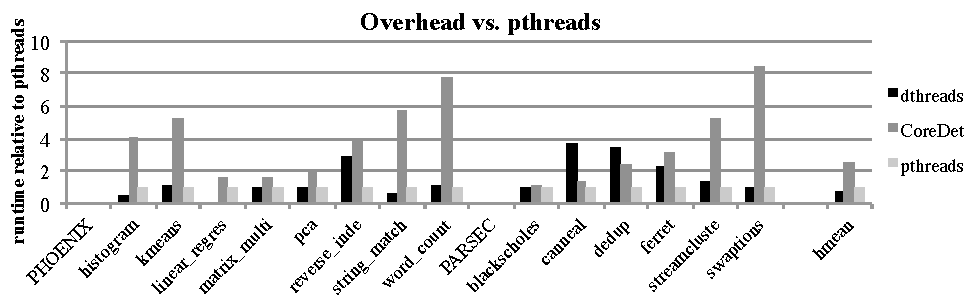
\includegraphics[width=6in]{dthreads/figure/overhead-figure}
\caption{Normalized execution time with respect to \pthreads{} and CoreDet(lower is better). For 9 of the 14 benchmarks, \dthreads{} runs nearly as fast or faster than \pthreads{}, while providing deterministic behavior.\label{fig:performance}}
}
\end{figure*}

\begin{table*}[!t]
\centering
\resizebox{\columnwidth}{!}{
\begin{tabular}{l|rrr|rr|l}
{\bf \small Benchmark} & {\bf \small CoreDet} & {\bf \small \dthreads{}} & {\bf \small \pthreads{}} & $\frac{\mbox{\bf \small CoreDet}}{\mbox{\bf \small \pthreads{}}}$ & $\frac{\mbox{\small \bf \dthreads{}}}{\mbox{\small \bf \pthreads{}}}$ & {\bf \small Input} \\

\hline
{\bf \small histogram} & 0.97 & 0.73 & 0.35 & $1.32\times$ & $0.48\times$ & {\it \small large.bmp} \\
{\bf \small kmeans} & 68.41 & 13.16 & 15.02 & $5.20\times$ & $1.14\times$ & {\it \small -d 3 -c 1000 -p 100000 -s 1000} \\ 
{\bf \small linear\_regression} & 6.42 & 4.11 & 0.57  & $1.56\times$ & $0.14\times$ & {\it \small key\_file\_500MB.txt} \\
{\bf \small matrix\_multiply} & 31.68 & 19.32 & 19.28  & $1.63\times$ & $0.99\times$ & {\it \small 2000 2000 } \\
{\bf \small pca} & 39.24 & 20.49 & 21.14  & $1.92\times$ & $1.03\times$ & {\it \small -r 4000 -c 4000 -s 100 } \\
{\bf \small reverse\_index} & 7.85 & 2.06 & 6.53 & $3.81\times$ & $3.17\times$ & {\it \small datafiles} \\
{\bf \small string\_match} & 18.31 & 3.19 & 1.97 & $5.74\times$ & $0.62\times$ & {\it \small key\_file\_500MB.txt} \\
{\bf \small word\_count} & 17.17 & 2.17 & 2.37 & $7.91\times$ & $1.09\times$ & {\it \small word\_100MB.txt} \\
{\bf \small blackscholes} & 10.49 & 9.47 & 9.30 & $1.11\times$ & $0.98\times$ & {\it \small 8 in\_1M.txt prices.txt} \\
{\bf \small canneal} & 14.74 & 10.41 & 39.82 & $1.42\times$ & $3.83\times$ &  {\it \small 7 15000 2000 400000.nets 128} \\
{\bf \small dedup} & 3.38 & 1.45 & 5.39 & $2.33\times$ & $3.72\times$ & {\it \small -c -p -f -t 2 -i media.dat output.txt} \\
{\bf \small ferret} & 21.89 & 7.02 & 26.86 & $3.11\times$ & $3.83\times$ & {\it \small corel lsh queries 10 20 1 output.txt} \\
{\bf \small streamcluster} & 14.33 & 2.74 & 4.61 & $5.23\times$ & $1.68\times$ &  {\it \small 10 20 128 16384 16384 1000 none output.txt 8} \\
{\bf \small swaptions} & 35.21 & 4.18 & 3.88 & $8.42\times$ & $0.93\times$ & {\it \small -ns 128 -sm 50000 -nt 8} \\
\hline
\end{tabular}
}
\caption{Benchmarks: execution time (in seconds) and input parameters.\label{tbl:benchmarks}}
\end{table*}

We next compare the performance of \dthreads{} to CoreDet
and \pthreads{}. Figure~\ref{fig:performance} presents these results graphically (normalized to \pthreads{}); Table~\ref{tbl:benchmarks} provides detailed information about execution time and input parameters.

\dthreads{} outperforms CoreDet on 12 out of 14 benchmarks (running between 20\% and $11.2\times$ faster). For 9 benchmarks, \dthreads{} runs nearly the same as or better
performance than \texttt{pthreads}. Because \dthreads{} isolates updates in separate processes, it can improve performance by eliminating false sharing: since concurrent ``threads'' actually execute in different physical pages, there is no coherence traffic caused by false sharing between synchronization points. \dthreads{} eliminates catastrophic false sharing in the \texttt{linear\_regression} benchmark, allowing it to execute over $7\times$ faster than \pthreads{} and $11\times$ faster than CoreDet. The \texttt{string\_match} benchmark exhibits a similar, though less dramatic, false sharing problem, allowing \dthreads{} to run almost 60\% faster than \pthreads{} and $9\times$ faster than CoreDet. Two benchmarks, \texttt{histogram} and \texttt{swaptions}, also run faster with \dthreads{} than with \pthreads{} ($2\times$ and $6\%$, respectively; $2.7\times$ and $9\times$ faster than with CoreDet). We believe but have not yet verified that the reason is false sharing.

For some benchmarks, \dthreads{} incurs modest overhead. For example, unlike most benchmarks examined here, which create long-lived threads, the \texttt{kmeans} benchmark creates and destroys over 1,000 threads in the course of its execution. 
While Linux processes are relatively lightweight, creating and exiting a process is still more expensive than the same operations of threads, accounting for a 14\% performance degradation of \dthreads{} over \pthreads{} (though it runs $4.6\times$ faster than CoreDet).

\dthreads{} runs substantially slower than \pthreads{} for 4 of the 14 benchmarks examined here. The \texttt{ferret} benchmark relies on an external library to analyze image files during the first stage in its pipelined execution model; this library makes intensive (and in the case of \dthreads{}, unnecessary) use of locks. Lock acquisition and release in \dthreads{} imposes higher overhead than ordinary \pthreads{} mutex operations. More importantly in this case, the intensive use of locks in one stage forces \dthreads{} to effectively serialize the other stages in the pipeline, which must repeatedly wait on these locks to enforce a deterministic lock acquisition order. The other three benchmarks (\texttt{canneal}, \texttt{dedup}, and \texttt{reverse\_index}) modify a large number of pages. With \dthreads{}, each page modification triggers a segmentation violation, a system call to change memory protection, the creation of a private copy of the page, and a subsequent copy into the shared space on commit (see Section~\ref{sec:future-work} for planned optimizations that may reduce this cost). We note that CoreDet also substantially degrades performance for these benchmarks, so much of this slowdown may be inherent to any deterministic runtime system.

\subsection{Scalability}
\label{sec:scalability}

\begin{figure}
{\centering
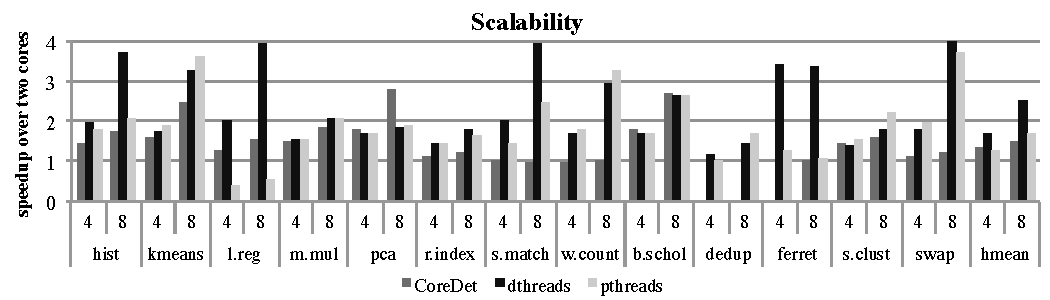
\includegraphics[width=6in]{dthreads/figure/scalability-figure}
\caption{Speedup of eight cores versus two cores (higher is better).  When possible to control with command line options, the number of threads was matched to the number of cores enabled.\label{fig:scalability}}
}
\end{figure}

To measure the scalability cost of running \dthreads{}, we ran two benchmark suite (excluding \texttt{canneal}) on the same machine with eight cores and again with two cores enabled.  Whenever possible without source code modifications, the number of threads was matched to the number of CPUs enabled.  We have found that \dthreads{} scales at least as well as \pthreads{} for 9 of 13 benchmarks, and scales as well or better than CoreDet for all but one benchmark where \dthreads{} outperforms CoreDet by 2x.  Detailed results of this experiment are presented in Figure~\ref{fig:scalability} and discussed below.

\texttt{canneal} was excluded from the scalability experiment because this benchmark does more work when more threads are present, making the performance comparison between eight and two threads unfair.  \dthreads{} hurts scalability relative to \pthreads{} for four of the benchmarks: \texttt{kmeans}, \texttt{word\_count}, \texttt{dedup}, and \texttt{streamcluster} although only marginally in most cases.  In all of these cases, \dthreads{} scales better than CoreDet.

\dthreads{} is able to match the scalability of \pthreads{} for three benchmarks: \texttt{matrix\_multiply}, \texttt{pca}, and \texttt{blackscholes}.  With \dthreads{}, scalability actually \emph{improves} over \pthreads{} for 6 out of 13 benchmarks: \texttt{histogram}, \texttt{linear\_regression}, \texttt{reverse\_index}, \texttt{string\_match}, \texttt{ferret}, and \texttt{swaptions}.




\subsection{Performance Analysis}

\subsubsection{Benchmark Characteristics}

The data presented in Table~\ref{tbl:characteristics} are obtained from the executions running on all 8 cores.  Column 2 shows the percentage of time spent in the serial phases.  In \dthreads{}, all memory commits and actual synchronization operations are performed in the serial phases.  The percentage of time spent in the serial phases thus can affect performance and scalability. Applications with higher overhead in \dthreads{} often spend a higher percentage of time in the
serial phases, primarily because they modify a large number of pages that need to be committed during those phases.

Column 3 shows the number of transactions in each application and Column 4 provides the average length of each transaction (ms).  Every synchronization, including locks, conditional variable, barriers, and thread exits, demarcate transaction boundaries in \dthreads{}.  For example, \texttt{reverse\_index}, \texttt{dedup}, \texttt{ferret}
and \texttt{streamcluster} perform numerous transactions whose
execution time is less than 1ms, imposing a performance penalty for these applications.  Benchmarks with longer (or fewer) transactions run almost the same speed as or faster than \texttt{pthreads}, including \texttt{histogram} or \texttt{pca}.  In \dthreads{}, longer transactions amortize the overhead of memory protection and copying.

Column 5 and 6 provides more detail on the costs associated with memory updates (the number and total volume of dirtied pages). From the table, it is clear why \texttt{canneal} (the most notable outlier) runs much slower with \dthreads{} than with \pthreads{}. This benchmark updates over three million pages, leading to large performance overhead caused by creating  private copies, handling protection faults, and committing modifications on those pages to the shared memory space. 

\textbf{Conclusion: }
Most benchmarks examined here contain either a small number of transactions, thus having long running transactions, and modify a modest number of pages during execution. For these applications, \dthreads{} is able to amortize its overhead: by eliminating false sharing, it can even run faster than \pthreads{}. However, for the few benchmarks that perform numerous short-lived transactions, or modify a large amount of pages, \dthreads{} can introduce substantial overhead.


\begin{table*}[!t]
\centering
\resizebox{\columnwidth}{!}{
\begin{tabular}{l|rrrrr}
& {\bf \small Serial Phase} & {\bf \small Transactions} & {\bf \small TransLength} & {\bf \small DirtyPages} & {\bf \small DirtyPages}
\\
{\bf \small Benchmark} & {\bf \small (\% of time)} & {\bf (\#)} & {\bf \small (ms)} & {\bf \small (\#)} & {\bf \small (GB)}\\
%\hline
%\multicolumn{6}{|c|}{\emph{Phoenix}} \\
\hline
\small \textbf{histogram} & 0 & 23 & 15.47 & 29 & 0 \\
\small \textbf{kmeans} & 0 & 3929 & 3.82 & 9466 & 0.04\\
\small \textbf{linear\_regression} & 0 & 24 & 23.92 & 17 & 0\\
\small \textbf{matrix\_multiply} & 0 & 24 & 841.2 & 3945 & 0.02\\
\small \textbf{pca} & 0 & 48 & 443 & 11471 & 0.04 \\
\small \textbf{reverseindex} & 17\% & 61009 & 1.04 & 451876 & 1.72\\
\small \textbf{string\_match} & 0 & 24 & 82 & 41 & 0 \\
\small \textbf{word\_count} & 1\% & 90 & 26.5 & 5261 & 0.02\\
%\hline
%\multicolumn{6}{|c|}{\emph{PARSEC}} \\
%\hline
\small \textbf{blackscholes} & 0 & 24 & 386.9 & 991 & 0\\
\small \textbf{canneal} & 26.4\% & 1062 & 43 & 3606413 & 13.75\\
\small \textbf{dedup} & 31\% & 45689 & 0.1 & 356589 & 1.36\\
\small \textbf{ferret} & 12.3\% & 484127 & 0.05 & 844184 & 3.21 \\
\small \textbf{streamcluster} & 18.4\% & 130001 & 0.04 & 131992 & 0.50\\
\small \textbf{swaptions} & 0 & 24 & 163 & 867 & 0\\
\hline
\end{tabular}
}
\caption{Benchmark characteristics.\label{tbl:characteristics}}
\end{table*}

\subsubsection{Performance Impact Analysis}
We further evaluate the performance impact of two important components of \dthreads: deterministic synchronization (sync-only) and memory protection(prot-only).

\emph{Sync-only}: This configuration enforces a deterministic synchronization order. However, the memory protection is not enabled so different processes access the shared memory directly. We want to use this to show the performance impact of load imbalance, caused by synchronization based scheduling.

\emph{Prot-only}: This configuration runs threads in isolation, with commits at synchronization points. The order of synchronization and memory commits are non-deterministic. This configuration eliminates false sharing, but also introduces the performance overhead of isolation and memory commits. In order to guarantee correct execution, we replaced those synchronizations as corresponding cross-processes synchronizations. The lazy twin creation and single-threaded execution optimizations are disabled here because they are unsafe without deterministic synchronization. Thus, this configuration actually evaluates the performance of using the \sheriff{} framework. 


\begin{figure*}[!t]
{\centering
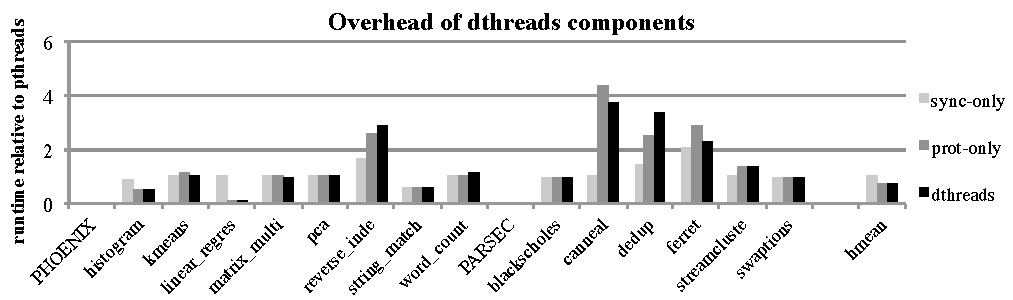
\includegraphics[width=6in]{dthreads/figure/perfeffect}
\caption{Normalized execution time with respect to \pthreads{} (lower is better) for three different configurations. 
\label{fig:perfanalysis}}
}
\end{figure*}

The performance results of these two configurations are shown in Figure~\ref{fig:perfanalysis} and discussed in the following.

\begin{itemize}

\item
The \texttt{reverse\_index}, \texttt{dedup} and \texttt{ferret} benchmarks show significant load imbalance under {\it sync-only} configuration. Additionally, these benchmarks introduces significant overhead with {\it prot-only} configuration because of a large number of transactions there. That explains why \dthreads{} doesn't have good performance on these benchmarks.

\item
The \texttt{string\_match} benchmark shows performance improvement with {\it sync-only} configuration. The exact reason is not clear, may be due to the per-thread allocator. 

\item
The \texttt{linear\_regression}, \texttt{histogram} and \texttt{swaptions} benchmarks improve performance with {\it prot-only} configuration. The memory isolation mechanism eliminates the false sharing problem inside and contributes to the performance speedup.

\item
Normally the performance of \dthreads{} is not better than the performance of {\it prot-only} configuration. However, both \texttt{ferret} and \texttt{canneal} run faster with determinism enabled. Both are benefited from specific optimization described in Section~\ref{sec:dthreads-optimization}. \texttt{ferret} benefits from the \emph{single-threaded-execution}. The performance improvement of \texttt{canneal} is coming from shared twin pages for all threads in the phase.

\end{itemize}






